\section{Figures Moved from the Main Text in v03}
\label{sec:moved_v03}
To keep the main paper at eight pages after adding the SpatialVLA results, three figures moved here; their numbers remain in the main text.

\begin{figure}[h]
\centering
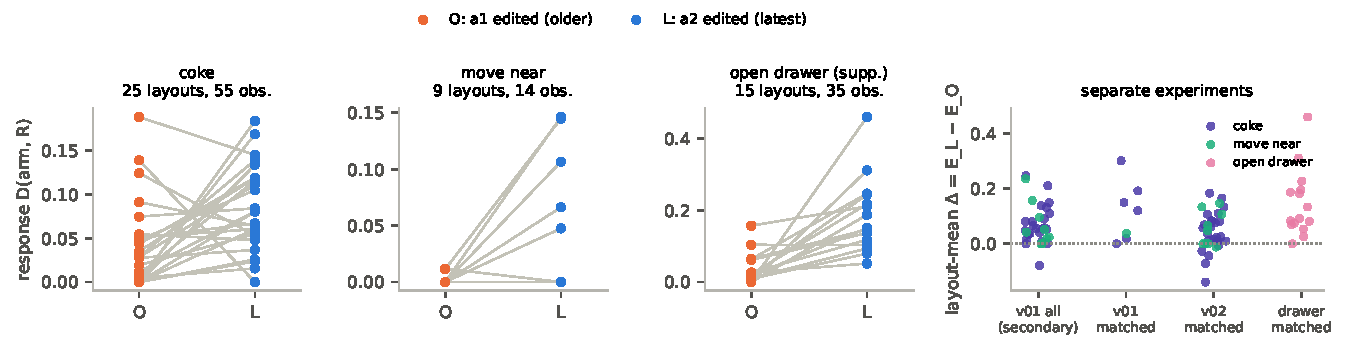
\includegraphics[width=\textwidth]{fig_svla_within_call.pdf}
\caption{\textbf{SpatialVLA within-call responses.} Left three panels: layout-mean responses to the older ($a_1$) and latest ($a_2$) edit in the matched follow-up (coke, move near) and the supplementary open-drawer task. Right: layout-mean $\Delta$ per experiment; experiments use different donor rules or tasks and are not pooled. Normalized action units, not metres.}
\label{fig:svla}
\end{figure}

\begin{figure}[h]
\centering
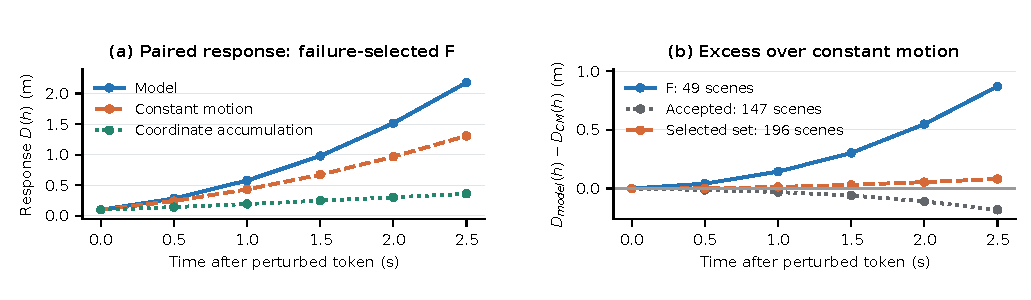
\includegraphics[width=\textwidth]{fig_time_resolved.pdf}
\caption{\textbf{AutoVLA: plan response beyond constant motion is concentrated in failure-selected plans.} Post-hoc curves under the original computation setting on a fixed common sample with perturbation position $t_p\leq4$: F has 342 units/49 scenes/13 drives; accepted has 1,032 units/147 scenes; their selected union has 19 drives. Left: paired response magnitudes in F. Right: excess over CM per stratum and in the union. Curves are scene means without inferential bands. Response magnitude is distinct from GT error.}
\label{fig:time}
\end{figure}

\begin{figure}[h]
\centering
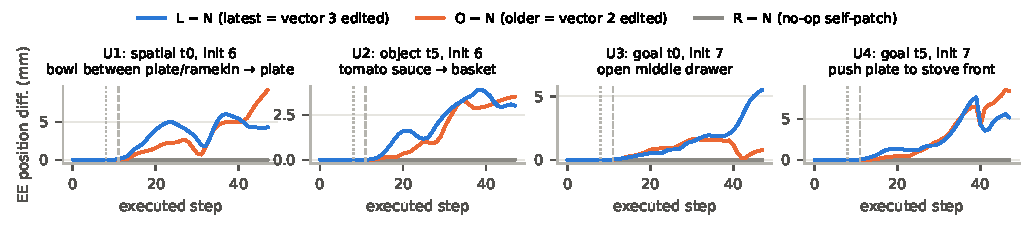
\includegraphics[width=\textwidth]{vla0_closed_loop_main.pdf}
\caption{\textbf{VLA-0: context-only edits change executed motion.} EE position difference (mm) from N after each executed step, for all four units and both edits (U1: spatial task 0, U2: object task 5, U3/U4: goal tasks 0/5; initial states 6/6/7/7). Dotted line: first edited call (step 8); dashed: first executed-command difference (step 11). R$-$N (gray) is zero. Command differences in control units are in Fig.~\ref{fig:vla0supp}.}
\label{fig:vla0cl}
\end{figure}
